\subsubsection{Rodzaje i zastosowanie  w grze cutscenek}
Po zebraniu feedbacku po playtestach część graczy zauważyła brak powiązania fabularnego między lokacją, do której trafia gracz a tytułem gry oraz stylistyką głównego menu.
Po przedyskutowaniu w obrębie zespołu postanowiliśmy stworzyć cutscenke wprowadzającą(intro), której zadaniem będzie stworzyć pomost między sceną na której znajduje się gracz, a tytułem.

Dodatkowo, postanowiliśmy również stworzyć odrębne cutscenki w ramach zakończenia rozgrywki (outro) - w dwóch wariantach,
w zależności czy gracz wygrał czy przegrał.
Z uwagi na decyzję o wdrożeniu również tutorialu w ramach cutscenki - polegającego na przeniesienie gracza na osobną scenę, która wcześniej była używana do testowania nowych mechanik - a następnie możliwość przejścia z poziomu samouczka do gry głównej - implementacja intro odbyła się na osobnej scenie z specjalnie przygotowanym środowiskiem którego przedstawienie znajduje się poniżej.
Takie rozwiązanie pozwoliło nam na zwiększenie ilości klatek na sekundę (FPS) podczas cutscenki - ze względu na brak konieczności renderowania oraz symulacji zachowania botów, pozbyciu się assetów broni, elementów interfejsu gracza, oraz samych mechanik powiązanych z graczem - takich jak poruszanie się, system ekwipunku, dynamiczna kamera (gracza jak i minimapy)

\subsubsection{Struktura sceny}
Do stworzenia scen outro - w obu wariantach - została wykorzystana scena \textbf{Game} - czyli scena główna na której odbywa się rozgrywka - ze względu na fakt że po zakończeniu rozgrywki, niezależnie od wygranej lub przegranej gracze - nic nie powstrzymuje nas przed usunięciem obiektów powiązanych z botami oraz graczem - oraz aktywowania obiektów stricte niezbędnych do scenki - gdyż rozgrywka sterowana przez gracza de facto dobiega końca.

Natomiast ze względu na wyżej opisane powody scena intro odbywa się na specjalnie przygotowanej scenie \textbf{Cutscene}.
Jej struktura pod kątem obecnych obiektów rozbita została na 3 główne sekcje:
\begin{itemize}
    \item Lokacja 1 - dom - wykorzystane tutaj zostało identyczne ułożenie obiektów jak do menu głównego.
    \item Lokacja 2 - teren - jest to kopia terenu głównego rozgrywki - zmniejszona o nieużywane elementy powiązane z rozgrywką
    \item Obiekty związane z samą scenką - najszersza kategoria. znajdują się tutaj wszystkie kamery wraz z dollyCartami,
    warstwa UI odpowiedzialna za wyświetlanie napisów przy dialogach, wszelkie efekty wizualne oraz obiekty animowane na osi czasu.
    Dodatkowo w tej kategorii znajdziemy wszelkie Managery wykorzystane do zarządzania przepływem pomiędzy scenami rozgrywki.
\end{itemize}

\subsubsection{Mechanizmy użyte w cutscence}
Rdzeniem naszych przerywników filmowych są dwie dostępne w samym Unity paczki - Cinemachine oraz Timeline.
Dodatkowo, bardzo ważną rolę odgrywa również paczka pozwalająca na sterowanie tekstami z TextMeshPro z poziomu timeline, stworzona przez Krisa Kreja.

Warto również wspomnieć o dubbingu, który został wygenerowany przy użyciu narzędzia \href{https://play.ht/}{AI text to speech}.
Poniżej screenshoty przedstawiające konkretne konfiguracje dla poszczególnych głosów:
\begin{figure}[h]
    \centering
    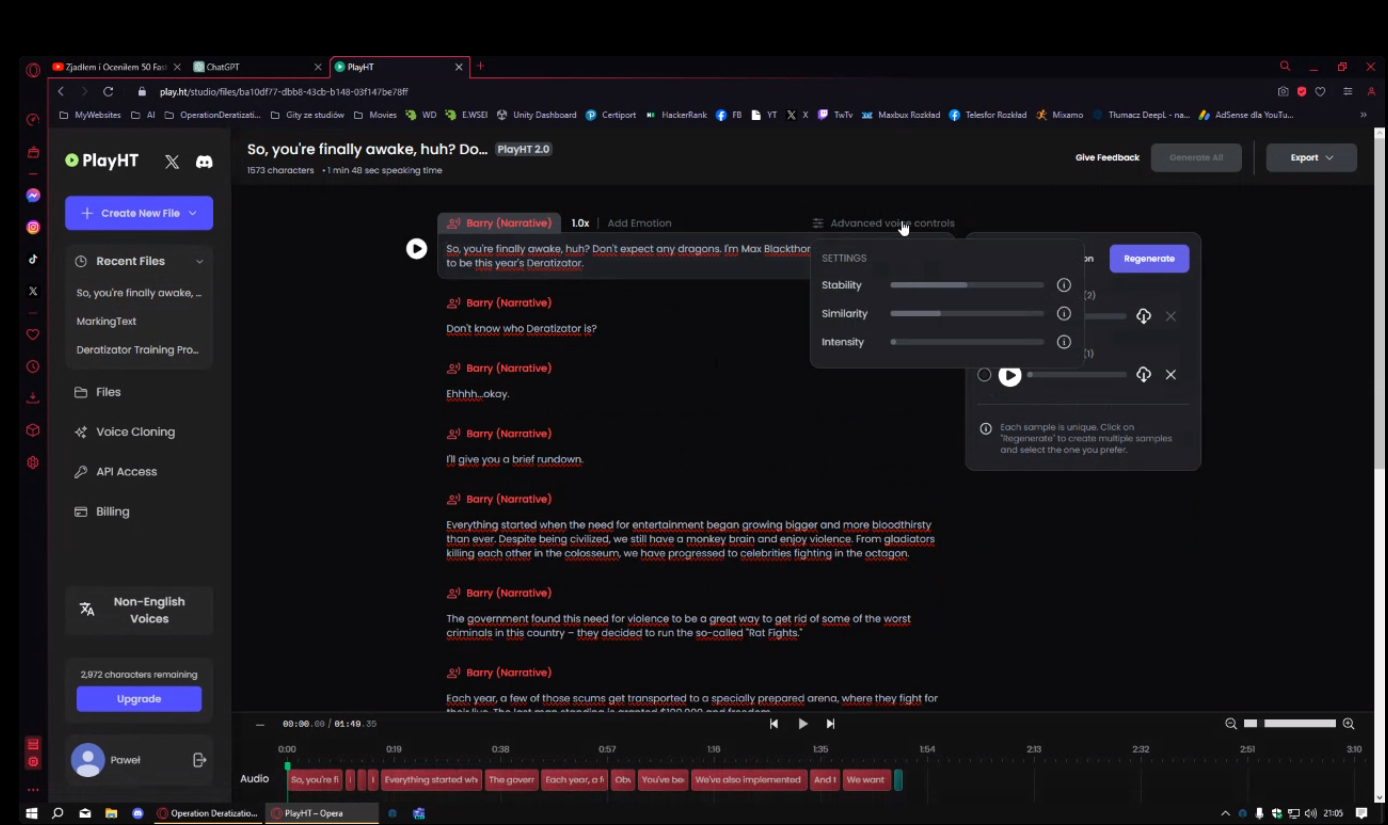
\includegraphics[width=1\linewidth]{Images/voice_max.PNG}
    \caption{Konfiguracja głosu dla Maxa - narratora pierwszej części intro}
\end{figure}
\begin{figure}[h]
    \centering
    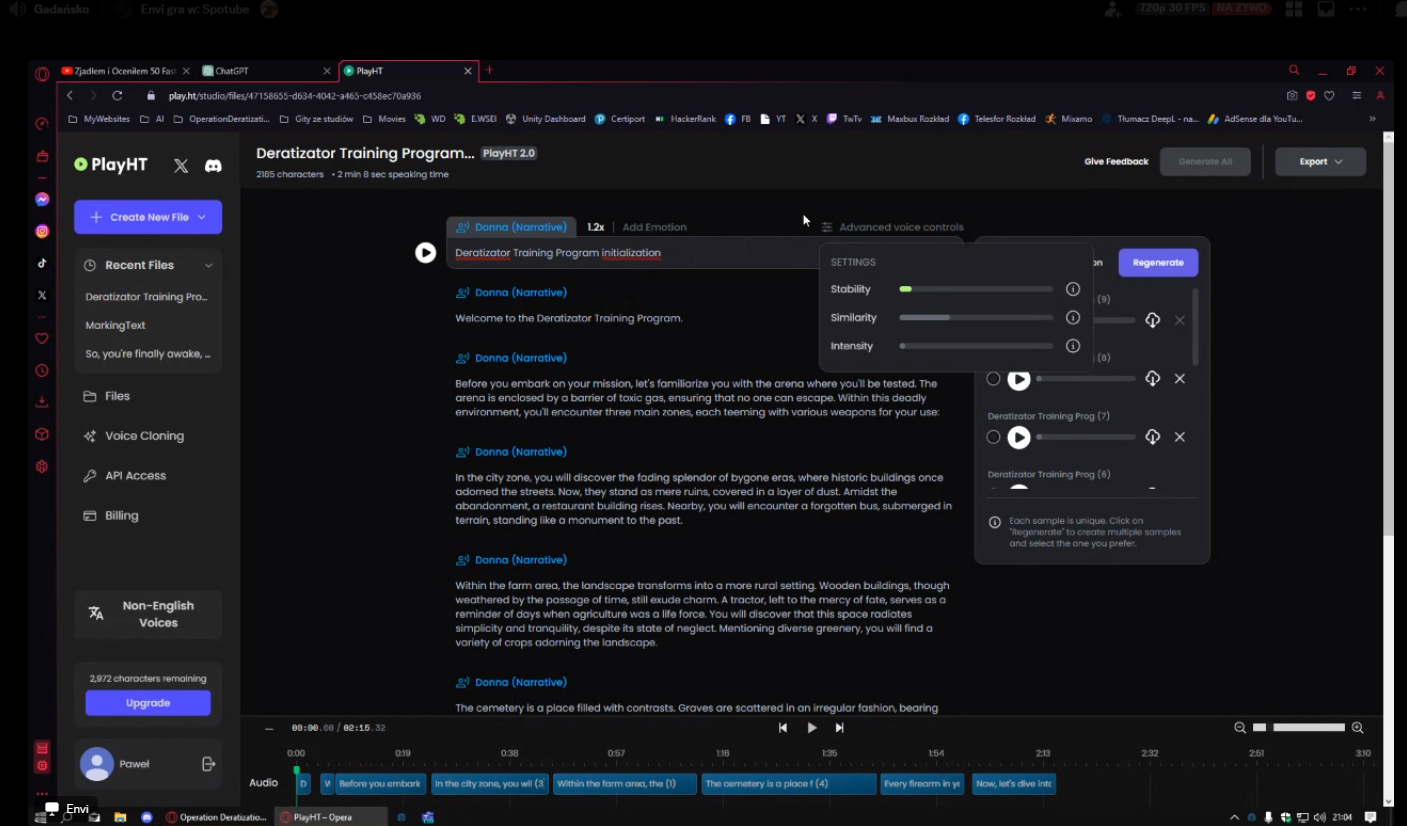
\includegraphics[width=1\linewidth]{Images/voice_intro_chip.png}
    \caption{Konfiguracja głosu dla narratora drugiej części intro - Smart Chip}
\end{figure}
\begin{figure}[h]
    \centering
    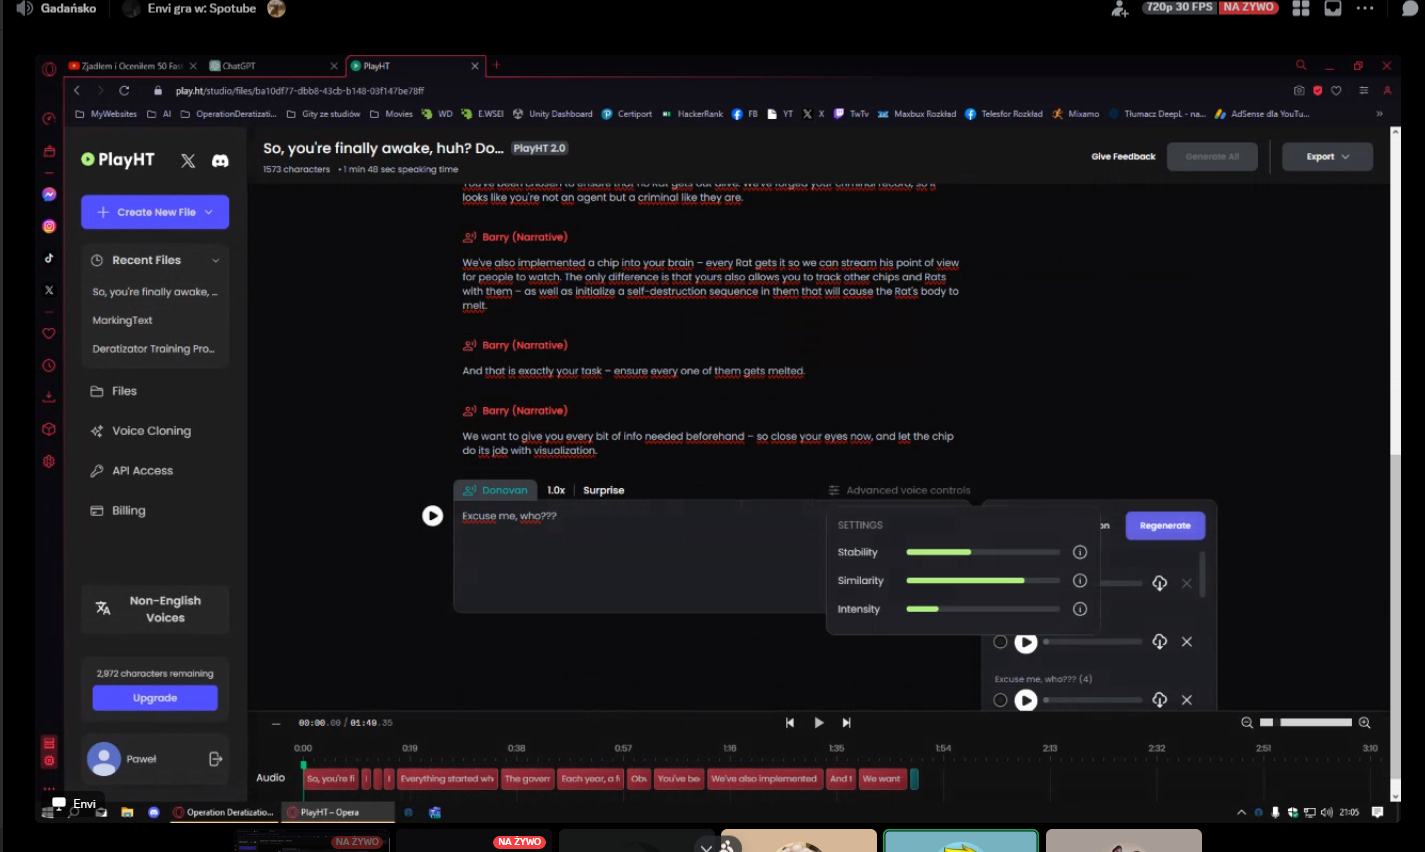
\includegraphics[width=1\linewidth]{Images/voice_hero.PNG}
    \caption{Konfiguracja głosu dla głównego bohatera}
\end{figure}
\FloatBarrier
Dialogi zostały rozdzielone na oddzielne pliki - po jednym zdaniu per linijka.
Po umieszczeniu na timeline wszystkich dialogów, dostosowane zostało poruszanie się postaci.
\subsubsection{Cutscenka Intro - pozostałe w trakcie pracy}

Zamysł cutscenki stanowi rozwinięcie fabuły przedstawionej tutaj \nameref{game_description} \\
Cutscenka Intro ze względu na swoją strukturę oraz historie przestawioną może zostać na dwie osobne sekcje - pierwszą, w domku, gdzie narratorem jest postać Maxa Blackthorna - którego osoba pozostaje dla gracza pewnego rodzaju zagadką, na podstawie dialogów można snuć domysł że jest to agent rządowy, który wdraża nas - graczy - w role którą pełnimy w rozgrywce.\\
Początek scenki informuje nas niebezpośrednio że wszystkie zdarzenia oglądane są z perspektywy postaci gracza - poprzez efekt zamykania i otwierania oka.\\
Efekt ten został osiągnięty poprzez 
Sugeruje nam to również że gracz mógł zostać porwany.
Następnie narrator odchodzi, a na ścianie za nim zostaje za pomocą animatora naniesiona grafika w Sprite2D - oraz aktywowane i dezaktywowane jest światło (Spot Light), co emituje efekt odtwarzania slajdów.
Pozostały fragment pierwszej części cutscenki sprowadza się do kolejnych linii dialogu oraz zmiany slajdów (wyłączanie i analogiczna animacja dla innych obiektów Sprite2D)\\
Końcowy dialog jest punktem przełomowy - gracz jest informowany o posiadaniu przez postać "chipa" w głowie - co stanowi uzasadnienie mechanik takich jak oznaczenie ciał przeciwników czy nawet użyty interface - dodatkowo wprowadzenie owego "chipu" jako postaci pozwala zmienić narratora i w naturalny sposób zaprezentować graczowi poziom - co odbywa sie w drugiej części intro\\
Druga część intro to pokazanie wszystkich lokacji oraz punktów zainteresowania - wraz z narracją wprowadzającą historie owych miejsc.\\
Głównym elementem zastosowanym w tej części cutscenki jest użycie wielu wirtualnych kamer oraz przełączanie się między nimi - oraz zmiana ich rotacji wraz z czasem z poziomu Animatora.\\
W celu poprawy wrażeń wizualnych niektóre z kamer posiadają zablokowany punkt na który patrzą (Look At) - dzięki czemu rozwiązanie polegające na pokazanie całego poziomu stało się znacznie łatwiejsze - kamera porusza się dookoła mapy, patrząc na pusty obiekt znajdujący się idealnie w centrum.\\
Na potrzeby tej części sceny zmodyfikowany również został skrypt odpowiedzialny za kontrolę drzwi:
\begin{codebox}
\begin{lstlisting}[language={[Sharp]C}, label={listing:DoorMotionSensor.cs}]
public class DoorMotionSensor : MonoBehaviour
{
    // ... (Remaining part of the script)
    
    if (isUsingCameraCheck)
    {
        float distanceToCamera = Vector3.Distance(transform.position, vCamera.transform.position);
        distance.Add(distanceToCamera);
        CinemachineTrackedDolly dollyCart = vCamera.GetCinemachineComponent<CinemachineTrackedDolly>();
        
        if (dollyCart != null)
        {
            float pathPosition = dollyCart.m_PathPosition;
            
            if (pathPosition >= 3f && pathPosition <= 4f || pathPosition >= 4.1f && pathPosition <= 5f)
                count++;
        }
    }
            
    // ... (Remaining part of the script)
}
\end{lstlisting}
\end{codebox}
\captionof{lstlisting}{Zmiany sposobu kontrolowania drzwi w skrypcie DoorMotionSensor.cs}
dzięki czemu obiekt DollyCart był w stanie aktywować animację otwierania drzwi podczas "wjazdu" kamery do restauracji, gdzie takowe drzwi zostały użyte.
Następnie zakończenie scenki prowadzi do przekierowania i wczytania sceny \textbf{Tutorial} - na której gracz może zapoznać się z mechanikami już z poziomu rozgrywki.